\chapter{Metode}
\label{chap:metode}
Under projektforløbet benyttede vi  en række metoder, der har til formål at strukturere og forbedre arbejdsprocessen. Vi benyttede den iterative, også kendt som evolutionære, arbejdsmetode fra første dag i projektet. Derudover brugte vi udvalgte metoder og aktiviteter fra Objektorienteret Analyse \& Design bogen \cite{ooad}, da vi mente, at de er gode til strukturering af rapportens indhold samt forløb. Feedback og kommentarer til alle dele af analyse, design, og modellering af systemet blev hentet fra to udvalgte informanter, som vi interviewede flere gange over de 4 måneder, projektet strakte sig over.

% Metoder skrevet ovenover:
%   - Evolutionære arbejdsmetode
%   - Aktiviteter fra bogen
%   - Informanter
% Er der mere?

\section{Evolutionær metode}
\label{sec:evolution}
\tjek{Revideret af Elias d. 9.12.12}

Det er vanskeligt at planlægge et helt projekt for et stort problem. Det kræver meget forarbejde, og man bliver nødt til at fortolke og revidere problemstillingen mange gange, indtil man har tilstrækkelig viden og forståelse for problemet. Dette gøres på bedste vis ved at have tæt kommunikation og interaktion med potentielle brugere af det fremtidige system. Vi har udviklet et system til brugerne, og det er dem, der skal bruge systemet. Derfor er det vigtigt, at de kan finde ud af at bruge systemet, og på samme tid udvikler vi en bedre forståelse for problemet igennem interaktionen med brugerne. 

Den evolutionære metode, bygger på en iterativ arbejdsproces, hvor der gennem hver iteration sker en udvikling i forståelsen af et problem. Metoden bygger på eksperimentering med bl.a. prototyper til at skabe sig en forståelse for problemet. Arbejdsmetodens iterationer, kaldes også for faser. I hver fase reviderer og bearbejder man analysen, designet af systemet, implementering og kvalitetssikringen. \cite{cic} Når vi siger, at vi har benyttet en iterativ arbejdsproces, så betyder det ikke, at der ikke også har været linæere tilgange i planlægningen. Men det betyder, at hvis man ser på den samlede udviklingsproces, så er det den iterative tilgang, der dominerer.

Projektet strakte sig over fire måneder, og vi vurderede, at fire faser af tre ugers varighed var en fornuftig opdeling af tiden, og at det gav os tilstrækkelig tid til hver fase. Disse fire faser kan ses i \tableref{table:iterationeroverblik}. Hver fase havde et formål, og et resultat. Tabellen har til formål at give læseren et hurtigt overblik over, hvad der er foregået i de forskellige faser. I tabellen står der eksempel hvilke dele af rapporten, der er blevet tilføjet eller revideret i den enkelte fase. I den første fase er der ikke noget at revidere, da vi ikke havde udført noget arbejde endnu. Derudover beskriver tabellen, hvordan vi har interageret med informanterne.

Informanterne, der bliver beskrevet i \secref{sec:samarbejde}, hjalp os bl.a. med at forstå problemet og hvordan en eventuel løsning på problemet skulle udformes. Vi holdt et initierende møde med dem, for at få en bred forståelse af problemet. Vi præsenterede informanterne for prototyper, der havde til formål at visualisere, hvilke tanker vi havde gjort os i forhold til en eventuel løsning, og vi ønskede at undersøge, hvordan informanterne interagerede med disse. Vi havde to prototyper, hvis fokus lå på søgefunktionaliteten i systemet og en prototype, hvis fokus lå på andre funktioner, systemet kunne have. Prototyperne er beskrevet yderligere i \secref{sec:samarbejde}. 


\ourtable{iterationeroverblik}{3}{Denne tabel giver et hurtigt og kortfattet overblik over projektets arbejdsfaser. Her ses de forskellige faser af den iterative arbejdsmetode med tilhørende formål og de resultater, vi har fået ud af de forskellige faser. Desuden kan man se, hvordan informanterne er blevet inddraget i processen.}
             {Beskrivelser}
       {Fase}  {Formål                       & Resultat                           & Informanternes inddragelse}{
\ourrow{1   }{At få indblik i informanternes problemstillinger, mht. madlavning og anvendelse af deres madrester, og at modellere disse. At definere et system, og forstå hvilke funktioner informanterne har brug for. & \textit{Tilføjet:} \textbf{Problmeområdet.} Klasser. Hændelser. Hændelsestabel. Klassestruktur. Prototype med fokus på søgefunktionalitet.  & Møde med fokus på problemet. Møde med fokus på løsning. Prototype med fokus på søgefunktionalitet.}
\ourrow{2   }{At sikre os, at de funktioner vi har i systemet passer med informanternes behov og at dokumentere og modellere disse. & \textit{Tilføjet:} \textbf{Problemområdet. Anvendelsesområdet.} Brugsmønstre. Funktioner. Aktører. Kriterier. Forbilleder. \textit{Revideret:} \textbf{Problemområdet.} Prototype med fokus på funktionalitet.  & Prototype med fokus på funktionalitet.}
\ourrow{3   }{At modellere systemet, ved at implementere funktioner og sikre os, at de definerede kriterier bliver opfyldt.     & \textit{Tilføjet:} \textbf{Implementering.} Sammensætning af rapport. Komponenter. Udtrækning af data i opskrifter. \textit{Revideret:} \textbf{Problemområdet. Anvendelsesområdet. Design.}  &  }
\ourrow{4   }{  At implementere det designede system.                                    & \textit{Tilføjet:} \textbf{Implementering. Kvalitetssikring.} \textit{Revideret:} \textbf{Problemområdet. Anvendelsesområdet. Design.}                                &           Bestemmelse af råvaretype fra ingrediens. 
Usability-test. }
}



% hvem er de
% hvad laver de
% hvad laver vi med dem

% hvad har de været ind over?
% inddrage, deltagelse

\section{Samarbejde med brugere}
\label{sec:samarbejde}

Vi mener, at systemet skal være rettet til brugerenes behøv og ønsker. Derfor valgte vi to informanter, som hver hører til to relative forskellige forbrugsområder hvilket gav et større indblik til andre forbrugere, som vi ikke kan nå. Vi har konsulteret vores 2 informanter med hensyn til inspiration og opklaring af gruppediskussioner. Hvis vi har været i tvivl om hverken en klasse eller struktur skulle indgå i systemet, tog vi kontakt til vores informanter for at høre deres meninger.

Informanter vil også være en stor del af afprøvnings- og kvalitetssikringsdelene af projektet. De skal være med til at sikre, at vi udvikler et system, der stemmer overens med systemdefinitionen og dækker deres behov med hensyn til madlavning i husstanden. Dette gr vived at udvikle forskellige prototyper, som vi præsenterer for informanterne til møderne . Diss prototyper repræsenterer de id\'{e}er, i har til en given funktion eller systemsdel, som vi ønsker at få feedback på.


\section{Prototyper}
\label{sec:prototyper}

Vi udarbejdede to prototyper, der fokuserede på søgefunktionaliteten, som bliver præsenteret i \secref{subsec:prototype1}, og en større prototype, der fokuserede på systemets andre funktioner, som bliver præsenteret i \secref{subsec:prototype2}.

Vi udførte prototypeafprøvningerne hjemme hos begge informanter (en af gangen). 
Informanterne blev bedt om at udføre en case, som havde til formål at få dem igennem prototyperne, så vi havde mulighed for at overvåge dem, og efterfølgende diskutere prototyperne med dem.
Afprøvningerne er dokumenteret ved hjælp af videooptagelser, som refereres til i \apref{ap:prototype1} for prototyperne, der havde fokus på søgefunktionalitet, og i \apref{ap:prototype2} for prototypen, der havde fokus på systemets andre funktioner.

Prototyperne med fokus på søgefunktionalitet blev afprøvet i første fase af projektforløbet, og prototypen med fokus på systemets andre funktioner blev afprøvet i anden fase, hvilket også er illustreret i \tableref{table:iterationeroverblik} i \secref{sec:evolution}.


\section{Prototype 1}
\label{ap:prototype1}

Afprøvning af Prorotype 1A på Merete er blevet filmet. Klippet kan ses på Youtube: \url{http://youtube.com/watch?v=E-8WA6QrZo4}

Afprøvning af Prorotype 1B på Merete er blevet filmet. Klippet kan ses på Youtube: \url{http://youtube.com/watch?v=rUJexwTpu48}

\begin{description}
\item[Formål] Vores system kan ikke benyttes uden at brugeren indtaster en mængde ingredienser, som de vil udføre en søgning på. For at tilbyde en brugervenlig metode til indtastning af disse ingredienser vil vi gerne teste 2 forskellige metoder på informanterne. Disse 2 metoder testes med hver deres prototype i papirsform, prototype 1A og 1B.
\item[Prototype 1A]

\begin{figure}[H]
\centering
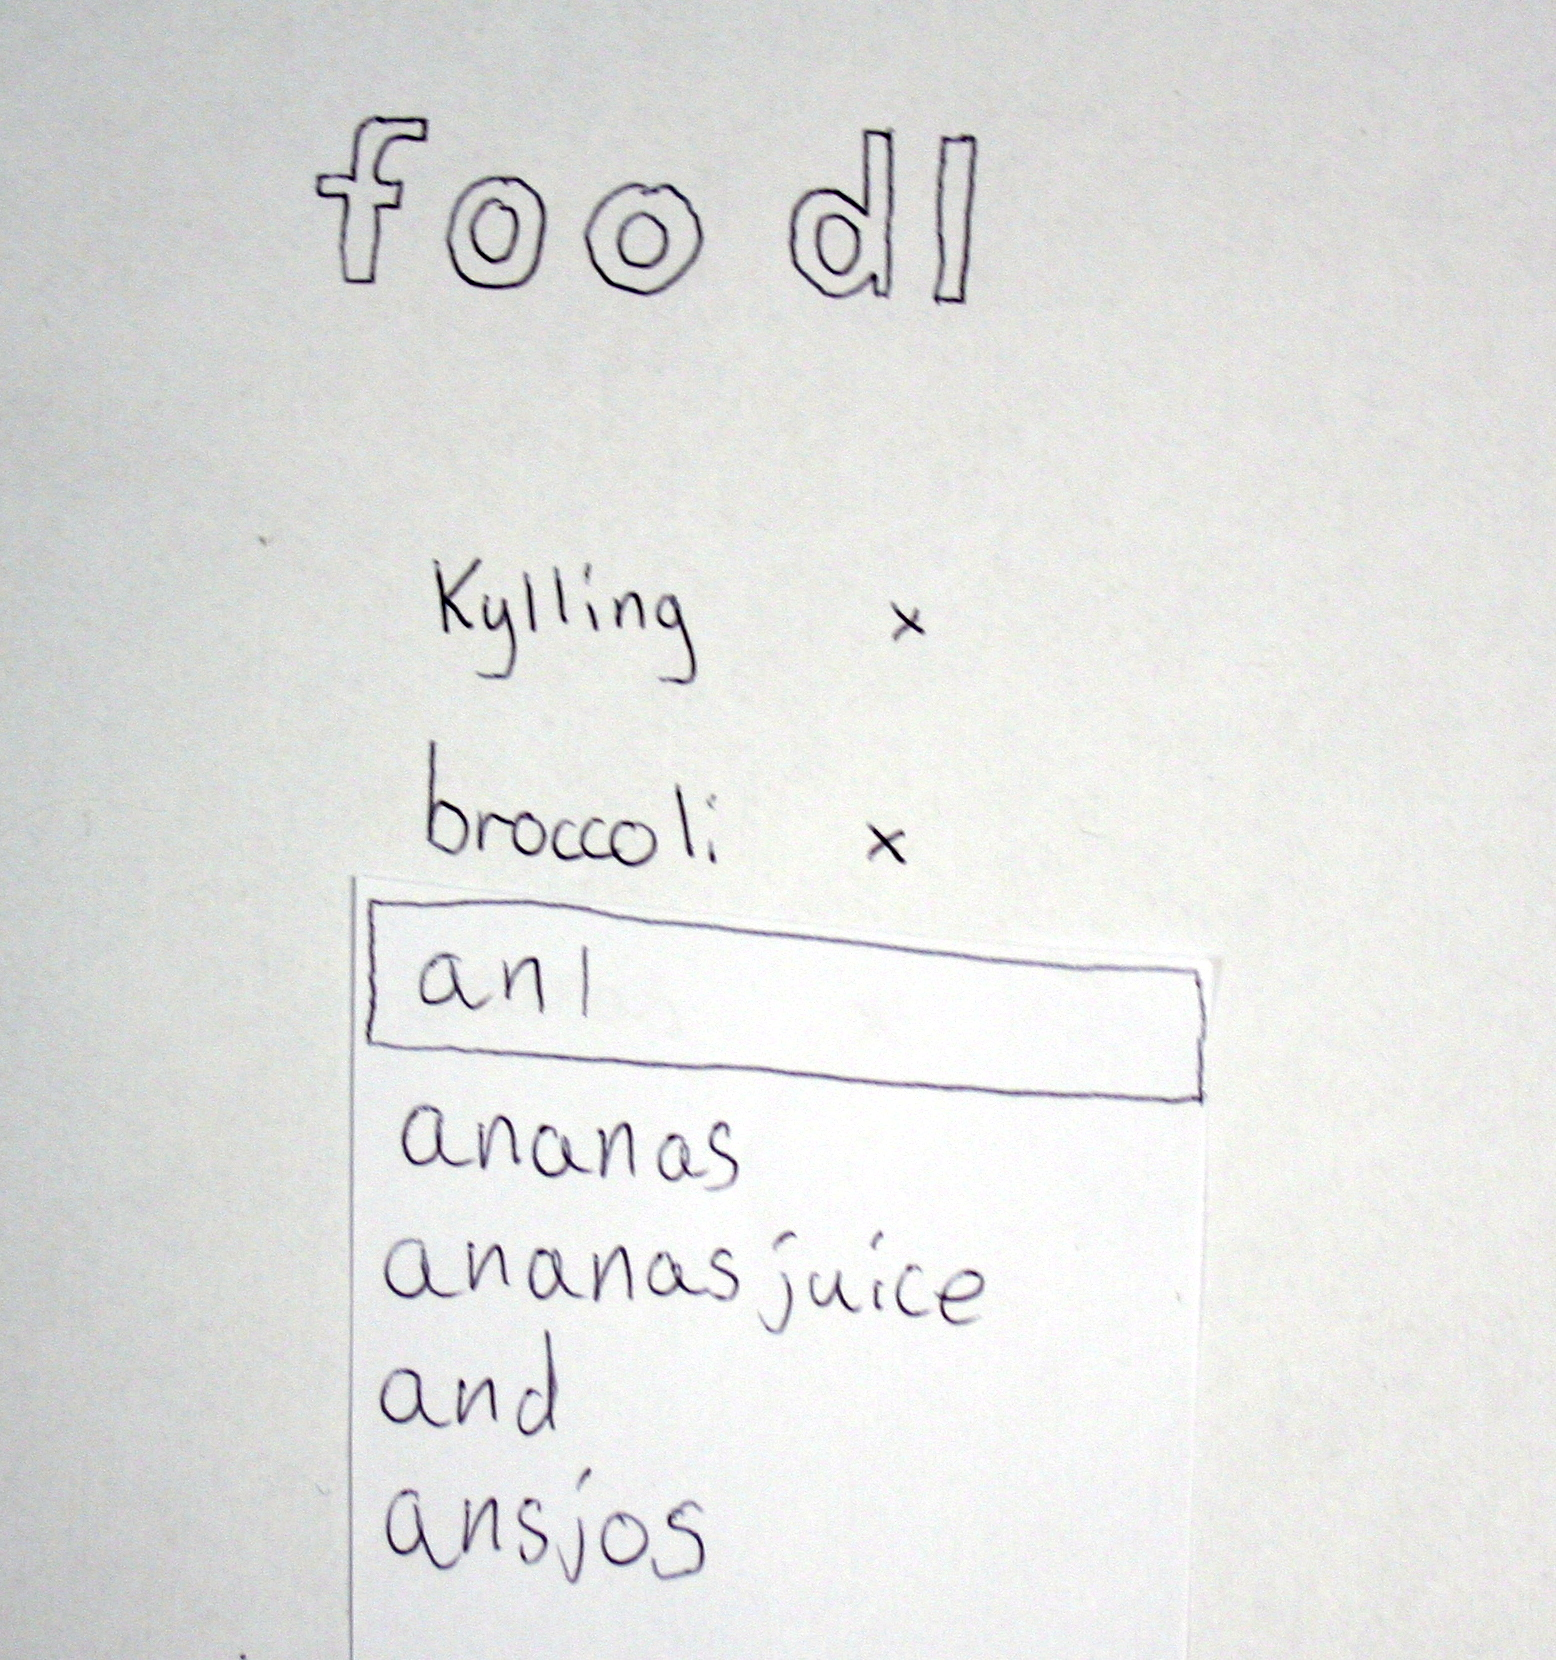
\includegraphics[width=0.5\textwidth]{billeder/prototyper/prototype1a.jpg}
\capt{Visualisering af prototype 1A.}
\label{fig:prototype1a}
\end{figure}

Præsenterer en søgeboks for brugeren, der minder meget om Google’s søgefelt. Når man indtaster et bogstav, fx “k”, kommer der en række forslag frem, såsom kylling og kartoffel, også på samme måde som ved Google, blot med den forskel at der kun foreslås ingredienser. Man kan nu klikke på forslaget eller trykke enter. Man kan også skrive ingrediensens navn færdig manuelt.

Tanken bag denne metode er at man hurtigt kan indtaste en ingrediens hvis man blot ved hvordan de første få bogstaver staves. Brugeren har med stor sandsynlighed kendskab til denne metode, da den bruges af Google, og samtidig har vi også konstrueret logoet og sidens design så det også minder om Google, netop for at gøre det intuitivt for brugeren.

Ulempen er at man har brug for et tastatur og skal tænke over hvordan man staver til ingrediensen. Det er også muligt at overse forslagene og tro man er nødsaget til at stave et meget langt ord, som for eksempel 

\item[Prototype 1B]

\begin{figure}[H]
\centering
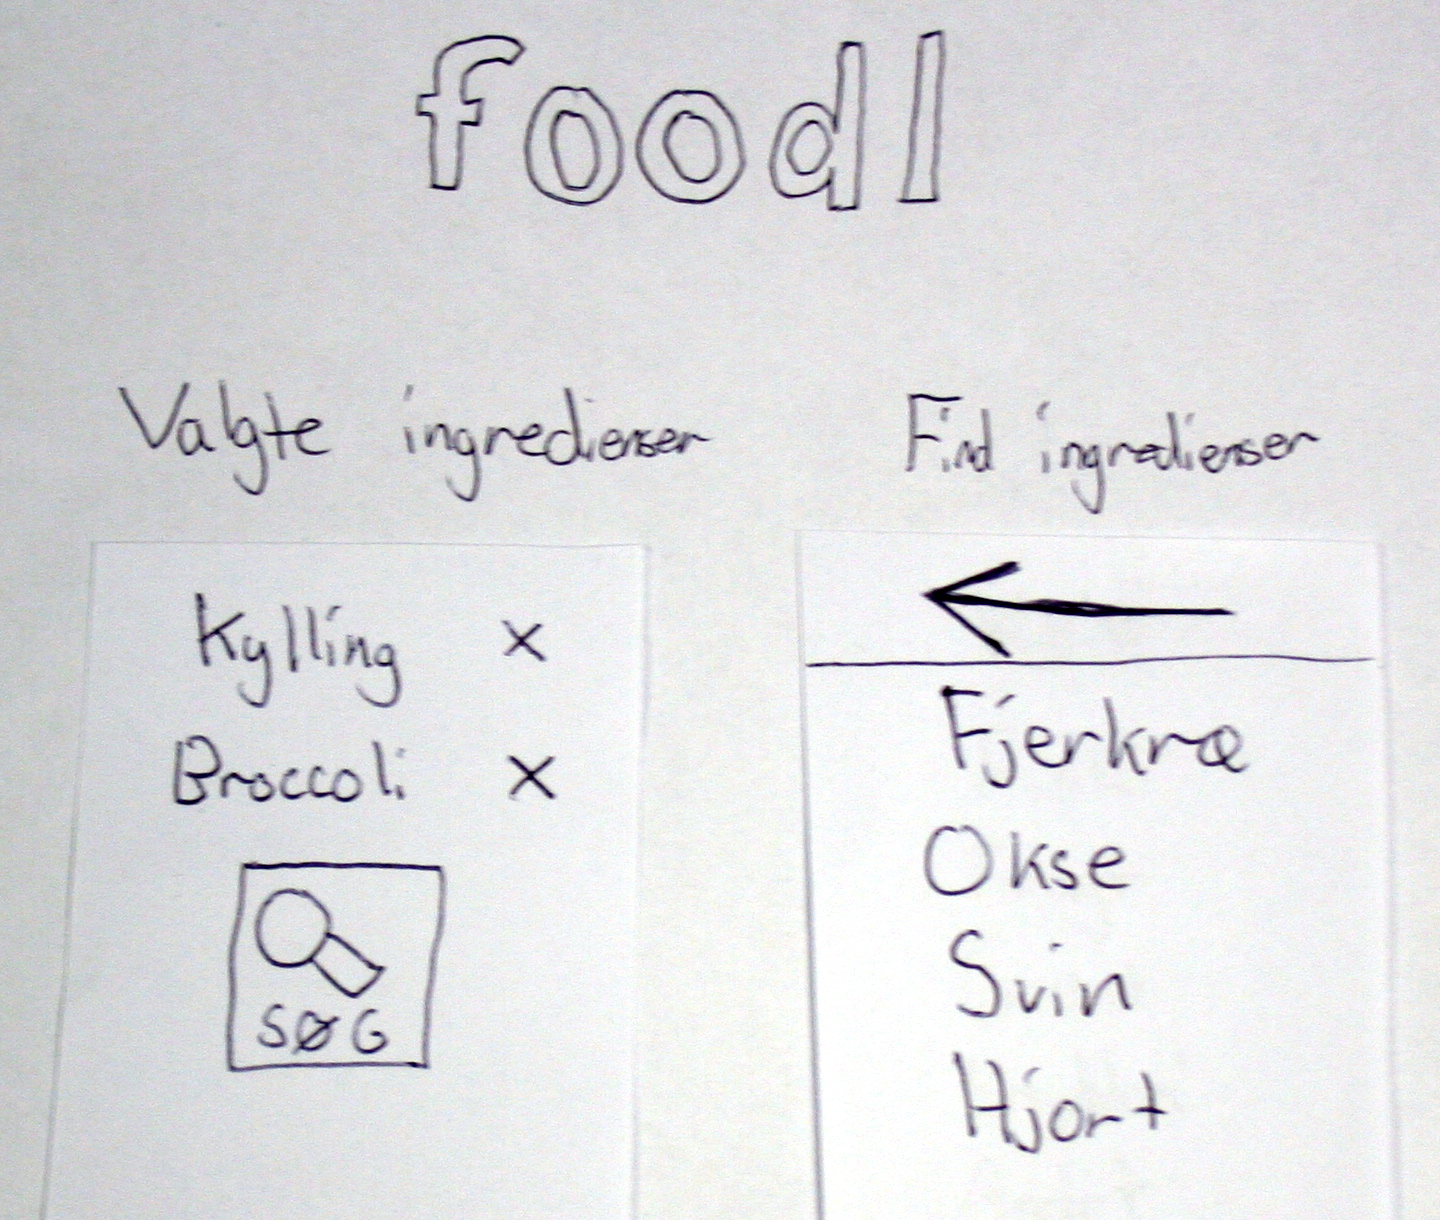
\includegraphics[width=0.5\textwidth]{billeder/prototyper/prototype1b.jpg}
\capt{Visualisering af prototype 1B.}
\label{fig:prototype1b}
\end{figure}

Fokuserer på et valg af ingredienser blandt kategorier. Man vælger først en bred kategori, som for eksempel fjerkræ, kød, brød, frugt og grønt. Dernæst vælger man et antal gange en underkategori, indtil man til sidst kan vælge en ingrediens fra en liste.

Fordelen ved denne metode er at brugeren ikke har behov for et tastatur. Det er også nemt at benytte på tablets og smartphones, da der kan skal klikkes. Ulempen er muligheden for mange kategori og forvirring omkring hvilken kategori en ingrediens findes i. Måske vil den sidste kategori der vælges stadig indeholde rigtig mange ignredienser, sådan at man skal bladre i denne liste for at finde den ønskede ingrediens. 

\item[Sammendrag] Prototype 1A var hurtig, nem og effektiv. Informanten kunne bedst lide denne metode, og hun havde ikke brug for vejledning for at kunne finde de 3 ingredienser kylling, ananas og broccoli.

Prototype 1B var langsommere at bruge og informanten syntes ikke om den. Hun var i tvivl om hvilken kategori hun skulle vælge kylling under. Kategorierne kan laves på mange forskellige måder, og uanset hvordan de vælges, vil der med garanti være nogle brugere der er i tvivl om hvor de skal lede efter en bestemt ingrediens. Et eksempel kan være kartoffelstivelse. Nogle vil lede efter kartoffelstivelse i kategorien grøntsager (fordi kartofler findes der), mens andre måske vil lede efter en kategori med navnet brød og gryn.

På baggrund af informantens valg, vælger vi at benytte metoden fra prototype 1A til at vælge ingredienser.
\end{description}

\section{Prototype 2}

Afprøvning af prototype 2 m/ fokus på systemets funktioner

\begin{description}
\item[Formål] På baggrund af møde 2, hvor informanterne kom med krav til systemets funktioner, har vi nu lavet en diasshow-prototype på gomockingbird.com, hvor systemets funktion er vist. Når informanterne præsenteres for funktionerne i noget der, med lidt god vilje, ligner et rigtigt program, så kan det være at informanten bliver klar over at en funktion enten mangler, eller at en tidligere foreslået funktion er overflødig. Formålet med mødet er derfor primært at ud af, om der er de funktioner, som informanten har brug for. Derudover vil vi også gerne finde ud af om brugeren kan finde de nødvendige funktioner, altså om programmet og dets funktioner som helhed er intuitive at bruge for informanterne.

\begin{figure}[H]
\centering
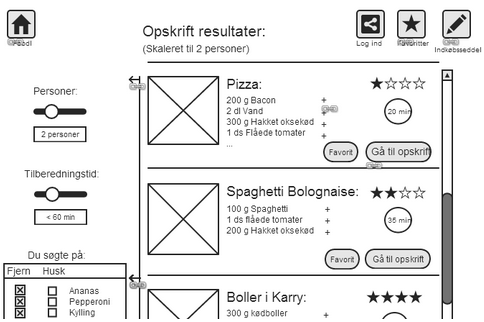
\includegraphics[scale=0.7]{billeder/prototyper/prototype2.png}
\capt{Visualisering af prototype 2.}
\label{fig:prototype2}
\end{figure}

Først udføres en case for at få ledt brugeren rundt blandt alle funktionerne.

\item[Case] Følgende case blev udført af informanterne.

\begin{enumerate}[noitemsep]
\item Udfør en søgning på ingredienserne (pepperoni, ananas og kylling). Ingredienser tilføjes ved at klikke i søgefeltet
\item Skjul alle opskrifter med nødder
\item Gå til den første opskrift, der fremkommer
\item Gå tilbage og tilføj 200 g Bacon (fra pizzaens ingredienser) til din indkøbsliste
\item Print indkøbslisten ud
\item Gør klar til en helt ny søgning
\item Foretag en søgning på pepperoni
\item Du fandt ingen opskrifter, så du vil gerne tilføj ananas, inden du søger igen (du søger altså på pepperoni og ananas)
\item Føj den første opskrift, du finder, til dine favoritter
\end{enumerate}

Efter casen tages en snak om hver af disse funktioner og muligheder med systemet.

Informanten bliver præsenteret for mange funktioner, hvor vi her beskriver hvad deres mening var omkring disse funktioner efter at have udført casen.

\begin{itemize}[noitemsep]
\item Begrænse søgeresultat efter tilberedningstid
\begin{itemize}[noitemsep]
\item Merete synes idéen er god, men foreslår nu kun 2 valgmuligheder ``kort'' eller ``lang'' tilberedningstid
\item Keld synes også dette er en god ide. En opdeling på en 30 min. burde være fint, måske 15 min. Hvis det er tilberedningstid på over en time, må skalaen godt springe mere end 15-30 min.
\end{itemize}
\item Sidebar
\begin{itemize}[noitemsep]
\item Merete opdagede ikke at denne sidebar kunne trækkes ud
\item Den ligger ikke logisk for en. Selvom den er stor. Den bliver skjult i designet
\item Keld synes ikke det ser for rodet ud, selvom sidebaren er ude hele tiden
\end{itemize}
\item Skalere en opskrift til x personer
\begin{itemize}[noitemsep]
\item Merete ser det som en nyttig funktion, hun vil skalere til mellem 2-4 personer
\item Det er en god funktion, som Keld er sikker på mange vil få brug for. Opskalering til 5 burde være nok. Måske 1-20, så er gæstebehov også dækket ind. Men det er trods alt til rester, så til 5 personer burde være nok.
\end{itemize}
\item Fjerne ingredienser inden en søgning udføres (på forsiden)
\begin{itemize}[noitemsep]
\item Merete synes det er meget brugbart
\item Keld synes det er fint at det er på forsiden
\end{itemize}
\item Fjerne ingredienser efter en søgning er udført (på søgeresultatsiden)
\begin{itemize}[noitemsep]
\item Merete synes idéen med at kunne fjerne ingredienser mens der vises søgeresultater er god
\item Keld synes det er fint, at det også er muligt i sidebaren
\end{itemize}
\item Huske ingredienser til næste søgning
\begin{itemize}[noitemsep]
\item Merete synes måden det fungerer på i prototypen er god. Hun vil ikke have at de huskede ingredienser vises på forsiden
\item Keld synes det er rart at det er muligt at huske nogle ingredienser. Det ville måske også være rart, hvis det også var muligt at gøre fra forsiden. Keld er dog i tvivl om, hvor på forsiden det skulle være. Det er måske alligevel bedst hvis forsiden er simpel. Han synes funktionen er brugbar
\end{itemize}
\item Skjule opskrifter indeholdende bestemte ting
\begin{itemize}[noitemsep]
\item Merete synes det virker godt
\item Keld synes det er en god ide. Han fik hurtigt fundet funktionen, så snart toolboxen blev åbnet
\end{itemize}
\item Browsers tilbageknap går til forsiden (beholder ingredienser)
\begin{itemize}[noitemsep]
\item Merete opdagede ikke denne funktion
\item Keld opdagede funktionen, og anvendte den også. Måske ville en tilbage- og fremknap på selve siden være brugbar, foreslår Keld
\end{itemize}
\item Home knap går tilbage (fjerne ingredienser)
\begin{itemize}[noitemsep]
\item Merete synes det virkede naturligt
\item Keld synes det er godt at have en kanp som går helt tilbage. Men han foreslår endnu engang at have en frem- og tilbageknap som supplerer home-knappen
\end{itemize}
\item Visning af opskrifter (ekspander ved mouse over)
\begin{itemize}[noitemsep]
\item Merete synes opskrifterne blev vist fint. Hun kunne godt lide idéen med at ekspandere opskriften ved mouseover
\item Keld synes bare man skal have vist de væsentligste ingredienser. Han synes det ville være smart, hvis det var muligt at se hele ingredienslisten ved hjælp af et mouse-over
\end{itemize}
\item Gå til opskrifter (evt link ved klik på navn)
\begin{itemize}[noitemsep]
\item Merete synes ikke knappen “Gå til opskrift”, er overflødig. Hun ville blive forvirret hvis den ikke var der, og man bare skulle trykke et sted på opskriften (navnet, eller baggrunden, hvor baggrundsfarve ændrer sig eller lignende)
\item Keld synes det er godt med en “Gå til opskrift”-knap. Det er brugervenligt
\end{itemize}
\item Tilføj opskrift til favoritter
\begin{itemize}[noitemsep]
\item Merete synes ikke man skal gå fra et søgeresultat og over til favoritsiden hver gang man tilføjer en opskrift til favoritter. Opskriften skal blot tilføjes. Måske den skal sige en lyd og fjerne knappen man trykkede på. Favoritter-ikonet kunne lyse op
\item Skal lave en “Fjern fra favorit-knap”, så man hurtigt kan ombestemme sig
\item Keld synes det er smart nok at man sendes ind på favoritlisten, så man er sikker på at opskriften er kommet derind. Havde man samtidig en frem- og tilbageknap ville det være endnu bedre
\end{itemize}
\item Favoritter (knappen, der viser ens favoritter)
\begin{itemize}[noitemsep]
\item Merete var lidt forvirret med hensyn til om den tilføjede en opskrift til favoritter, eller hvad den gjorde
\item Keld synes at det skal være muligt at skalere opskrifterne på favoritsiden og at det er muligt nemt at fjerne opskrift fra favoritsiden igen
\end{itemize}
\item Visning af favoritter (layout)
\begin{itemize}[noitemsep]
\item Merete syntes layoutet var godt, og kunne godt lide at det mindede om layoutet ved visning af søgeresultat
\item Keld synes godt om layoutet
\end{itemize}
\item Visning af indkøbsliste
\begin{itemize}[noitemsep]
\item Merete synes det er en god idé at man kan tilføje tekst
\item Keld foreslår at man har ingredienslisten fra den opskrift man har været inde på, ved siden af indkøbslisten, så det er muligt hurtigt at tilføje flere ingredienser derfra
\item Keld synes indkøbslisten er meget brugbar. Det er for ofte man glemmer nogle ting, uden indkøbslisten
\end{itemize}
\item Tilføje opskrifts ingredienser til indkøbsliste
\begin{itemize}[noitemsep]
\item Merete vidste ikke hvordan man gjorde. Hun troede ikke man kunne trykke på +’et
\item Keld kunne godt tilføje en ingrediens til indkøbslisten
\end{itemize}
\item Home-knappen sender en til en helt tom forside
\begin{itemize}[noitemsep]
\item Merete kunne godt lide dette. Det virkede helt naturligt for hende
\item Keld synes det giver mening
\end{itemize}
\item Logge ind (få afklaret med brugeren, hvordan det skal foregå)
\begin{itemize}[noitemsep]
\item Log ind mest forståeligt
\item Kender meget til login, intet til synkronisering
\item Log ind er klart mest forståeligt for Keld. Keld har ikke lyst til at indtaste mere end mail-adresse, navn eller brugernavn og adgangskode. Helst ikke mere end det. Det er fint at der kommer en bekræftelsesmail til ens indbakke, men helst ikke aktiveringsmail
\item Sikkerheden har ikke høj-prioritet for Keld, da der alligevel ikke er nogle følsomme informationer på siden
\end{itemize}
\item Informants forslag til flere funktion
\begin{itemize}[noitemsep]
\item Merete havde ingen forslag, udover at der skal være billede af opskrifterne, hvilket ikke var vist i prototypen
\item Keld foreslår at sidebaren også er på favoritsiden
\item Keld foreslår en frem- og tilbageknap
\item Filtrering af forskellige landes køkkener, så det eksempelvis var muligt at se italienske retter, kinesiske retter osv. (kun de mest kendte køkkener: nordiskekøkken, kinesiske, italienske, græske \fx)
\end{itemize}
\end{itemize}
\end{description}

\subsection{Sammendrag}

I forhold til funktionalitet i prototypen, er der nogle få ting, der skal tilføjes, fjernes eller ændres

\begin{enumerate}[noitemsep]
\item Når man på søgesiden tilføjer en opskrift til favoritter, skal man forblive på søgesiden. Knappen man trykkede på skal erstattes med en ``Fjern fra favoritter''-knap
\item Sidebaren på søgeresultatssiden skal være nemmere at få øje på. En løsning er at gøre den synlig fra starten og give brugeren muligheden for at skjule den
\item Knappen i toppen, der viser de favoritter man har gemt, skal være mere sigende. ``Vis favoritter'' kunne der stå under den
\item På søgeresultatsiden, hvor en opskrifts vises, skal +’et ud for ingredienserne, der tilføjer en ingrediensen til indkøbslisten, være mere intuitiv
\item Brugeren skal muligvis have at vide, at man kan benytte browserens tilbageknap for at gå tilbage til forsiden, uden at ingredienser fjernes. Det kan være at informanten overså denne funktion fordi prototypen blev vist i form af et diasshow på en hjemmeside, og informanten derfor var bange for at gå væk fra hele diasshowets side
\item Skalering og andre funktioner til visning af favoritter
\item Frem og tilbage knap, der giver brugeren tryghed når han navigerer rundt, så man ikke skal være bange for at browseren forsvinder fra siden
\end{enumerate}


